
\حصہ{میکس ویل مساوات کا عمومی حل}
اس حصے میں مستطیلی گھمکی مکمل طور پر حل کی جائے گی۔امید کی جاتی ہے کہ آپ اس طریقے کو پسند کریں گے۔

کثافت چارج سے خالی \عددیء{\rho_h=0} خطے کے میکس ویل کے مساوات
\begin{align}
\nabla \times \kvec{H}&=\sigma \kvec{E}+\epsilon \frac{\partial \kvec{E}}{\partial t} \label{مساوات_مویج_مستطیلی_گھمکیا_الف}\\
\nabla \times \kvec{E}&=-\mu \frac{\partial \kvec{H}}{\partial t} \label{مساوات_مویج_مستطیلی_گھمکیا_ب}\\
\nabla \cdot \kvec{H}&=0 \label{مساوات_مویج_مستطیلی_گھمکیا_پ}\\
\nabla \cdot \kvec{E}&=0 \label{مساوات_مویج_مستطیلی_گھمکیا_ت}
\end{align}
 سے شروع کرتے ہیں۔مساوات \حوالہ{مساوات_مویج_مستطیلی_گھمکیا_ب} کی گردش لیتے ہوئے حاصل جواب میں مساوات \حوالہ{مساوات_مویج_مستطیلی_گھمکیا_الف} اور مساوات \حوالہ{مساوات_مویج_مستطیلی_گھمکیا_ت} پر کرنے سے موج کی مساوات 
\begin{align*}
\nabla \times \nabla \times \kvec{E}=\nabla \left(\nabla \cdot \kvec{E}\right)-\nabla^2 \kvec{E}&=-\mu \frac{\partial }{\partial t}\left(\nabla \times \kvec{H}\right)\\
-\nabla^2 \kvec{E}&=-\mu \sigma \frac{\partial \kvec{E}}{\partial t}-\mu\epsilon \frac{\partial^2 \kvec{E}}{\partial t^2}
\end{align*}
حاصل ہوتی ہے۔یہ سمتی مساوات حقیقت میں تین مساوات کو ظاہر کرتی ہے۔ان میں سے  \عددیء{E_x} کی مساوات یوں
\begin{align*}
\nabla^2 E_x&=\mu \sigma \frac{\partial E_x}{\partial t}+\mu\epsilon \frac{\partial^2 E_x}{\partial t^2}
\end{align*}
یا
\begin{align}\label{مساوات_مویج_مستطیلی_گھمکیا_ٹ}
\frac{\partial^2 E_x}{\partial x^2}+\frac{\partial^2 E_x}{\partial y^2}+\frac{\partial^2 E_x}{\partial z^2}&=\mu \sigma \frac{\partial E_x}{\partial t}+\mu\epsilon \frac{\partial^2 E_x}{\partial t^2}
\end{align}
لکھی جائے گی جہاں برقی میدان \عددیء{E_x(x,y,z,t)} کے چار آزاد متغیرات ہیں۔\اصطلاح{علیحدگی متغیرات}\فرہنگ{علیحدگی متغیرات}\حاشیہب{separation of variables} استعمال کرتے ہوئے  برقی میدان کو دو تفاعل کے حاصل ضرب کے برابر لکھا جاتا ہے
\begin{align}\label{مساوات_مویج_مستطیلی_گھمکیا_ث}
E_x(x,y,z,t)=M(x,y,z) T(t)
\end{align} 
جہاں پہلے تفاعل \عددیء{M} کے تین آزاد متغیرات \عددیء{x}، \عددیء{y} اور \عددیء{z} ہیں جبکہ دوسرے تفاعل \عددیء{T} کا صرف \عددیء{t} آزاد متغیرہ ہے۔یوں مساوات \حوالہ{مساوات_مویج_مستطیلی_گھمکیا_ٹ} سے
\begin{align*}
T\left(\frac{\partial^2 M}{\partial x^2}+\frac{\partial^2 M}{\partial y^2}+\frac{\partial^2 M}{\partial z^2}\right)&=M\left(\mu \sigma \frac{\partial T}{\partial t}+\mu\epsilon \frac{\partial^2 T}{\partial t^2}\right)
\end{align*}
حاصل ہوتا ہے۔ دونوں اطراف کو \عددیء{MT} سے تقسیم کرتے ہوئے
\begin{align*}
\frac{1}{M}\left(\frac{\partial^2 M}{\partial x^2}+\frac{\partial^2 M}{\partial y^2}+\frac{\partial^2 M}{\partial z^2}\right)&=\frac{1}{T}\left(\mu \sigma \frac{\partial T}{\partial t}+\mu\epsilon \frac{\partial^2 T}{\partial t^2}\right)
\end{align*}
حاصل ہوتا ہے۔اس مساوات کا بایاں ہاتھ خلاء کے متغیرات \عددیء{x}، \عددیء{y} اور \عددیء{z} پر منحصر ہے جبکہ دایاں ہاتھ وقت \عددیء{t} پر منحصر ہے۔یوں خلاء کے متغیرات تبدیل کرنے سے صرف بایاں ہاتھ تبدیل ہونے کا امکان ہے لیکن بائیں ہاتھ میں تبدیلی کے بعد مساوات کے دونوں اطراف برابر نہیں ہوں گے لہٰذا یہ لازم ہے کہ مساوات کے دونوں اطراف قابل تبدیل نہ ہوں۔یوں انہیں مستقل \عددیء{k^2} کے برابر لکھا جا سکتا ہے یعنی
\begin{align*}
\frac{1}{M}\left(\frac{\partial^2 M}{\partial x^2}+\frac{\partial^2 M}{\partial y^2}+\frac{\partial^2 M}{\partial z^2}\right)&=\frac{1}{T}\left(\mu \sigma \frac{\partial T}{\partial t}+\mu\epsilon \frac{\partial^2 T}{\partial t^2}\right)=-k^2
\end{align*}
جس سے دو مساوات 
\begin{align}
\mu\epsilon \frac{\partial^2 T}{\partial t^2}+\mu \sigma \frac{\partial T}{\partial t}+k^2 T=0\label{مساوات_مویج_مستطیلی_گھمکیا_ج}\\
\frac{\partial^2 M}{\partial x^2}+\frac{\partial^2 M}{\partial y^2}+\frac{\partial^2 M}{\partial z^2}+k^2 M=0\label{مساوات_مویج_مستطیلی_گھمکیا_چ}
\end{align}
حاصل ہوتے ہیں۔

مساوات \حوالہ{مساوات_مویج_مستطیلی_گھمکیا_ج} کا حل \عددیء{T=e^{pt}} فرض کرتے ہوئے
\begin{align*}
\left(\mu\epsilon p^2+\mu \sigma p+k^2 T\right)e^{pt}=0
\end{align*}
سے
\begin{align*}
p=\frac{-\sigma\mp \sqrt{\sigma^2-4\frac{\epsilon}{\mu}k^2}}{2\epsilon}
\end{align*}
حاصل ہوتا ہے۔کامل ذو برق کی صورت میں \عددیء{\sigma=0} ہو گا جس سے
\begin{align}
p=\mp \frac{j k}{\sqrt{\mu \epsilon}} 
\end{align}
حاصل ہوتا ہے۔یوں
\begin{align*}
T(t)=c_t e^{ \mp\frac{j k}{\sqrt{\mu \epsilon}} t}
\end{align*}
ہو گا جہاں \عددیء{c_t} مساوات کا مستقل ہے۔اس میں
\begin{align}\label{مساوات_مویج_میکس_ویل_عمومی_تعدد}
\omega=\frac{ k}{\sqrt{\mu \epsilon}}
\end{align}
لیتے ہوئے مساوات کی جانی پہچانی شکل
\begin{align}
T(t)=c_t e^{ \mp j\omega t}
\end{align}
حاصل ہوتی ہے۔

مساوات \حوالہ{مساوات_مویج_مستطیلی_گھمکیا_چ} کو بھی علیحدگی متغیرات کے طریقے سے حل کرتے ہیں۔یوں
\begin{align}\label{مساوات_مویج_مستطیلی_گھمکی_علیحدگی_الف}
M(x,y,z)=X(x)N(y,z)
\end{align}
لیتے ہوئے
\begin{align*}
N\frac{\partial^2 X}{\partial x^2}+X\frac{\partial^2 N}{\partial y^2}+X\frac{\partial^2 N}{\partial z^2}+k^2 XN=0
\end{align*}
یا
\begin{align*}
\frac{1}{X}\frac{\partial^2 X}{\partial x^2}=-\frac{1}{N}\left(\frac{\partial^2 N}{\partial y^2}+\frac{\partial^2 N}{\partial z^2}\right)-k^2 
\end{align*}
حاصل ہوتا ہے جسے نئے مستقل \عددیء{-k_x^2} کے برابر لکھا جا سکتا ہے۔یوں 
\begin{align}
\frac{\partial^2 X}{\partial x^2}+k_x^2 X&=0 \label{مساوات_مویج_میکس_ویل_عمومی_الف}\\
\frac{\partial^2 N}{\partial y^2}+\frac{\partial^2 N}{\partial z^2}+(k^2 -k_x^2)N &=0
\end{align}
حاصل ہوتے ہیں۔ان میں دوسرے مساوات میں \عددیء{N} کو مزید دو تفاعل کا حاصل ضرب
\begin{align}\label{مساوات_مویج_مستطیلی_گھمکی_علیحدگی_ب}
N(y,z)=Y(y)Z(z)
\end{align}
 لکھتے ہوئے
\begin{align*}
Z\frac{\partial^2 Y}{\partial y^2}+Y\frac{\partial^2 Z}{\partial z^2}+(k^2 -k_x^2)YZ &=0
\end{align*}
یا
\begin{align*}
\frac{1}{Y}\frac{\partial^2 Y}{\partial y^2}=-\frac{1}{Z}\frac{\partial^2 Z}{\partial z^2}-k^2 +k_x^2
\end{align*}
لکھا جا سکتا ہے۔اس کو نئے مستقل \عددیء{-k_y^2} کے برابر  پر کرتے ہوئے دو مساوات
\begin{align}
\frac{\partial^2 Y}{\partial y^2}&=-k_y^2 Y \label{مساوات_مویج_میکس_ویل_عمومی_ب}\\
\frac{\partial^2 Z}{\partial z^2}&=-(k^2 -k_x^2-k_y^2)Z=-k_z^2 Z \label{مساوات_مویج_میکس_ویل_عمومی_پ}
\end{align}
حاصل ہوتے ہیں جہاں آخری قدم پر \عددی{(k^2 -k_x^2-k_y^2=k_z^2)} یا
\begin{align}\label{مساوات_مویج_مستطیلی_گھمکی_علیحدگی_پ}
k^2 =k_x^2+k_y^2+k_z^2
\end{align}
لیا گیا ہے۔مساوات \حوالہ{مساوات_مویج_میکس_ویل_عمومی_الف}، مساوات \حوالہ{مساوات_مویج_میکس_ویل_عمومی_ب} اور مساوات \حوالہ{مساوات_مویج_میکس_ویل_عمومی_پ} کے حل
\begin{align}
X&=c_xe^{\mp j k_x x}   \label{مساوات_مویج_گھمکی_عمومی_الف}\\
Y&=c_y e^{\mp j k_y y}   \label{مساوات_مویج_گھمکی_عمومی_ب}\\
Z&=c_z e^{\mp j k_z z}   \label{مساوات_مویج_گھمکی_عمومی_پ}
\end{align}
ہیں۔

مساوات \حوالہ{مساوات_مویج_مستطیلی_گھمکی_علیحدگی_الف}، مساوات \حوالہ{مساوات_مویج_مستطیلی_گھمکی_علیحدگی_ب} اور مساوات \حوالہ{مساوات_مویج_مستطیلی_گھمکیا_ث} سے ظاہر ہے کہ
\begin{align}\label{مساوات_مویج_گھمکی_عمومی_ت}
E_x(x,y,z,t)=X Y Z T=E_{x0} e^{j (\mp \omega t \mp k_x x \mp k_y y \mp k_z z)} 
\end{align}
کے برابر ہے جہاں مساوات کے مستقل کو \عددیء{E_{x0}} لکھا گیا ہے۔مساوات \حوالہ{مساوات_مویج_گھمکی_عمومی_ت} میکس ویل مساوات کا عمومی حل ہے جو کسی ایک خطے میں ہر ممکنہ \عددیء{E_x} موج کو ظاہر کرتی ہے۔اصل موج اس مساوات کا حقیقی  جزو ہو گا۔

اگر \عددیء{k_x=k_y=0} جبکہ \عددیء{\omega} اور \عددیء{k_z} مثبت قیمتیں ہوں تب 
\begin{equation}\label{مساوات_مویج_میکس_ویل_بڑھتے_جانب}
E_x= E_{x0} e^{j (\omega t -k_z z)} \quad \left\{
\begin{IEEEeqnarraybox}[][c]{l}
\IEEEstrut
\omega > 0 \\
k_z >0 \quad \text{\RL{بڑھتے $z$ جانب موج}}
\IEEEstrut
\end{IEEEeqnarraybox}
\right .
\end{equation}
کا حقیقی جزو
\begin{align}\label{مساوات_مویج_گھمکی_عمومی_ٹ}
E_x = E_{x0} \cos (\omega t -k_z z)
\end{align}
بڑھتے \عددیء{z} جانب موج ظاہر کرتی ہے جبکہ 
\begin{align}\label{مساوات_مویج_میکس_ویل_گھٹتے_جانب}
E_x= E_{x0} e^{j( \omega t +k_z z)}
\quad \left\{
\begin{IEEEeqnarraybox}[][c]{l}
\IEEEstrut
\omega > 0 \\
k_z >0 \quad \text{\RL{گھٹتے $z$ جانب موج}}
\IEEEstrut
\end{IEEEeqnarraybox}
\right .
\end{align}
گھٹتے \عددیء{z} جانب موج ظاہر کرتی ہے۔اسی طرح  چونکہ \عددیء{\cos (-\omega t -k_z z)=\cos(\omega t +k_z z)} ہوتا ہے لہٰذا
\begin{align}\label{مساوات_مویج_میکس_ویل_عمومی_زاویائی_الف}
E_x= E_{x0} e^{j(- \omega t -k_z z)}
\end{align}
بھی گھٹتے \عددیء{z} جانب موج کو ظاہر کرتی ہے۔آپ دیکھ سکتے ہیں کہ تفاعل \عددیء{T=c_t e^{j\omega t}} یا \عددیء{T=c_t e^{-j\omega t}} لیتے ہوئے  کسی بھی موج کو لکھا جا سکتا ہے۔فرق صرف اتنا ہے کہ پہلی صورت میں \عددیء{Z=c_z e^{-j k_z z}} لیتے ہوئے  بڑھتے \عددیء{z} جانب موج حاصل ہوتی  ہے جبکہ دوسری صورت میں \عددیء{Z=c_z e^{j k_z z}} لیتے ہوئے بڑھتے \عددیء{z} جانب موج حاصل ہوتی ہے۔ہم \عددیء{T=c_t e^{j\omega t}} چنتے ہوئے آگے بڑھتے ہیں۔اگر \عددیء{k_z} کی قیمت مثبت ہونے کے علاوہ منفی بھی ہو سکے تب مساوات \حوالہ{مساوات_مویج_میکس_ویل_بڑھتے_جانب} اور مساوات \حوالہ{مساوات_مویج_میکس_ویل_گھٹتے_جانب} کو ایک ہی مساوات
\begin{align}\label{مساوات_مویج_میکس_ویل_دونوں_جانب}
E_x= E_{x0} e^{j( \omega t -k_z z)}
\quad \left\{
\begin{IEEEeqnarraybox}[][c]{l}
\IEEEstrut
\omega > 0 \\
-\infty <k_z<+\infty  \quad \text{\RL{بڑھتے یا گھٹتے $z$ جانب موج}}
\IEEEstrut
\end{IEEEeqnarraybox}
\right .
\end{align}
کی صورت میں لکھا جا سکتا ہے جہاں مثبت قیمت کا \عددیء{k_z} بڑھتے \عددیء{z} جانب موج کو ظاہر کرتا ہے۔یوں مساوات \حوالہ{مساوات_مویج_گھمکی_عمومی_ت} کو 
\begin{align}\label{مساوات_مویج_گھمکی_عمومی_ث}
E_x(x,y,z,t)=E_{x0} e^{j (\omega t - k_x x - k_y y - k_z z)} 
\quad \left\{
\begin{IEEEeqnarraybox}[][c]{l}
\IEEEstrut
\omega > 0 \\
-\infty <k_x<+\infty \\
-\infty <k_y<+\infty \\
-\infty <k_z<+\infty 
\IEEEstrut
\end{IEEEeqnarraybox}
\right .
\end{align}
بھی لکھا جا سکتا ہے۔

کارتیسی محدد میں کسی بھی نقطہ \عددیء{(x,y,z)} کو سمتیہ
\begin{align}\label{مساوات_مویج_گھمکی_عمومی_ج}
\kvec{r}=x\ax+y\ay+z\az
\end{align}
ظاہر کرتی ہے۔ہم \عددیء{k_x}، \عددیء{k_y}، \عددیء{k_z}  اور \عددیء{k} کو سمتیہ
\begin{align}\label{مساوات_مویج_گھمکی_عمومی_چ}
\kvec{k}=k_x \ax+k_y \ay +k_z \az
\end{align}
لکھ سکتے ہیں جو مساوات \حوالہ{مساوات_مویج_مستطیلی_گھمکی_علیحدگی_پ} کے شرط پر پورا اترتی ہے۔اس طرح 
\begin{align}\label{مساوات_مویج_گھمکی_عمومی_ح}
\kvec{k} \cdot \kvec{r}=k_x x +k_y y +k_z z
\end{align}
ہو گا لہٰذا مساوات \حوالہ{مساوات_مویج_گھمکی_عمومی_ث} کو نہایت عمدگی کے ساتھ
\begin{align}\label{مساوات_مویج_گھمکی_عمومی_خ}
E_x=E_{x0} e^{j(\omega t-\kvec{k} \cdot \kvec{r})}
\end{align}
لکھا جا سکتا ہے جس کا حقیقی جزو
\begin{align}\label{مساوات_مویج_گھمکی_عمومی_د}
E_x=E_{x0} \cos (\omega t -\kvec{k} \cdot \kvec{r})
\end{align}
اصل موج دیتا ہے۔مندرجہ بالا مساوات لامحدود خطے میں موج کی عمومی مساوات ہے۔مثبت \عددیء{k} کی صورت میں موج بڑھتے \عددیء{\vec{k}} کی جانب حرکت کرے گی۔مساوات \حوالہ{مساوات_مویج_گھمکی_عمومی_خ} کی جگہ
\begin{align*}
E_x=E_{x0} e^{j(\omega t+\kvec{k} \cdot \kvec{r})}
\end{align*}
بھی لکھا جا سکتا ہے جہاں منفی \عددیء{k} کی صورت میں موج بڑھتے \عددیء{\vec{k}} کی جانب حرکت کرے گی۔ہم مساوات \حوالہ{مساوات_مویج_گھمکی_عمومی_د} استعمال کریں گے۔

کسی اٹل نقطے مثلاً \عددیء{z=z_0} پر مساوات \حوالہ{مساوات_مویج_گھمکی_عمومی_ٹ} وقت کے ساتھ سائن نما تعلق رکھتا ہے جس کی زاویائی تعدد \عددیء{\omega} ہے۔یوں ہم نے مساوات \حوالہ{مساوات_مویج_میکس_ویل_عمومی_تعدد} میں \عددیء{p} کی جگہ \عددیء{\omega} لکھ کر ٹھیک ہی کیا تھا۔

\begin{figure}
\centering
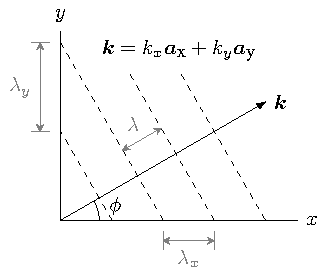
\includegraphics{figWaveguidesMaxwellGeneralWavelengthAndPropagationConstant}
\caption{مختلف طول موج کا آپس میں تعلق}
\label{شکل_مویج_مختلف_طول_موج}
\end{figure}

شکل \حوالہ{شکل_مویج_مختلف_طول_موج} میں موج کے حرکت کی سمت، \عددیء{x} محدد کے ساتھ \عددیء{\phi} زاویہ بناتی ہے۔اس شکل میں موج \عددیء{xy} سطح پر پائی جاتی ہے یعنی \عددیء{k_z=0} کے برابر ہے۔موج کی چوٹیوں کو نقطہ دار لکیروں سے ظاہر کیا گیا ہے۔کسی بھی نقطے پر ان چوٹیوں کو گن کر تعدد دریافت کی جا سکتی ہے۔یوں \عددیء{x} محدد پر نقطہ \عددیء{(x_0,0)} سے فی سیکنڈ گزرتے چوٹیوں کی تعداد \عددیء{f} موج کی تعدد ہو گی۔آپ دیکھ سکتے ہیں کہ \عددیء{y} محدد پر نقطہ \عددیء{(0,y_0)} سے بھی  فی سیکنڈ اتنی ہی چوٹیاں گزریں گی۔اسی طرح خط \عددیء{\kvec{k}} پر بھی کسی نقطے پر چوٹیاں گنتے ہوئے  یہی تعدد حاصل ہوتا ہے۔

دو متواتر چوٹیوں کے درمیان فاصلہ طول موج کہلاتا ہے۔ وقت \عددیء{t} کو روک کر \عددیء{x} محدد پر رہتے ہوئے موج کی دو متواتر چوٹیوں کے درمیان فاصلہ \عددیء{\lambda_x} ناپا جائے گا۔ اسی طرح \عددیء{y} محدد پر طول موج \عددیء{\lambda_y} ناپی جائے گی جبکہ حرکت کی سمت میں طول موج \عددیء{\lambda} ناپی جائے گی۔ان تمام کو شکل \حوالہ{شکل_مویج_مختلف_طول_موج} میں دکھایا گیا ہے۔

کسی بھی موج کی تعدد \عددیء{f} اور طول موج  \عددیء{\lambda} جانتے ہوئے اس کی رفتار \عددیء{v=f \lambda} لکھی جا سکتی ہے۔سمت حرکت کی جانب موج کی رفتار \عددیء{\tfrac{1}{\sqrt{\mu \epsilon}}} کے برابر ہوتی ہے لہٰذا
\begin{align}
f \lambda=\frac{1}{\sqrt{\mu \epsilon}}
\end{align}
ہو گا۔اس مساوات کے دونوں اطراف کو \عددیء{2\pi} سے ضرب دیتے ہوئے
\begin{align}
\lambda=\frac{2\pi}{\omega \sqrt{\mu \epsilon}}
\end{align}
حاصل ہوتا ہے جس میں مساوات \حوالہ{مساوات_مویج_میکس_ویل_عمومی_تعدد} پر کرنے سے
\begin{align}
\lambda=\frac{2\pi}{k}
\end{align}
یا
\begin{align}\label{مساوات_مویج_گھمکی_عمومی_ڈ}
k=\frac{2\pi}{\lambda}
\end{align}
حاصل ہوتا ہے لیکن \عددیء{\tfrac{2\pi}{\lambda}=\beta} ہوتا ہے۔ مندرجہ بالا مساوات کامل ذو برق \عددیء{\sigma=0} کے لئے حاصل کئے گئے لہٰذا \عددیء{\alpha=0}  اور
\begin{align}
\gamma=0+j\beta=j k
\end{align} 
کے برابر ہے۔اس طرح \عددیء{k} کو \عددیء{\beta} جبکہ \عددیء{k_x}، \عددیء{k_y} اور \عددیء{k_z} کو بالترتیب \عددیء{\beta_x}،\عددیء{\beta_y} اور \عددیء{\beta_z} لکھا جا سکتا ہے۔

ہم توقع کرتے ہیں کہ مساوات \حوالہ{مساوات_مویج_گھمکی_عمومی_ڈ} کی طرح \عددیء{\lambda_x=\tfrac{2\pi}{k_x}} لکھا جائے گا۔آئیں اس حقیقت کو ثابت کریں۔شکل  \حوالہ{شکل_مویج_مختلف_طول_موج} کو دیکھ کر \عددیء{\lambda_x=\tfrac{\lambda}{\cos \phi}} لکھا جا سکتا ہے جہاں شکل کو دیکھتے ہوئے \عددیء{\cos \phi=\tfrac{k_x}{k}} لکھا جا سکتا ہے۔یوں
\begin{align*}
\lambda_x=\frac{\lambda}{\cos \phi}=\frac{\lambda k}{k_x}
\end{align*}
لکھ کر \عددیء{k=\tfrac{2\pi}{\lambda}} پر کرتے ہوئے
\begin{align}
\lambda_x=\frac{2\pi}{k_x}
\end{align}
حاصل ہوتا ہے۔اسی طرح ہم 
\begin{align}
\lambda_y&=\frac{2\pi}{k_y}\\
\lambda_z&=\frac{2\pi}{k_z}
\end{align}
بھی حاصل کر سکتے ہیں۔

سمت حرکت کی جانب رفتار جسے \اصطلاح{مجموعی رفتار}\فرہنگ{رفتار!مجموعی}\حاشیہب{group velocity}\فرہنگ{velocity!group} کہتے ہیں
\begin{align}
v=f\lambda=\frac{\omega}{k}
\end{align}
کے برابر ہے۔موج اس رفتار سے توانائی ایک جگہ سے دوسری جگہ منتقل کرتی ہے۔اس کے برعکس کارتیسی محدد پر \اصطلاح{دوری رفتار}\فرہنگ{رفتار!دوری}\حاشیہب{phase velocity}\فرہنگ{velocity!phase} 
\begin{align*}
v_x&=f \lambda_x=\frac{\omega}{k_x}\\
v_y&=f \lambda_y=\frac{\omega}{k_y}\\
v_z&=f \lambda_z=\frac{\omega}{k_z}
\end{align*}
ہوں گے۔شکل \حوالہ{شکل_مویج_مختلف_طول_موج} میں \عددیء{\phi} کی قیمت کم کرنے سے \عددیء{\lambda_y} اور یوں \عددیء{v_y} کی قیمت بڑھتی ہے حتٰی کہ \عددیء{\phi=0} پر \عددیء{v_y=\infty} حاصل ہوتا ہے۔یوں دوری رفتار، روشنی کے رفتار سے زیادہ ہو سکتی ہے۔دوری رفتار  صرف آنکھوں کا دھوکہ ہے، اس رفتار سے موج کا کوئی حصہ حرکت نہیں کرتا لہٰذا یہ  آئن سٹائن کے قانون کی خلاف ورزی نہیں کرتا۔آئن سٹائن کا قانون کہتا ہے کہ کوئی چیز روشنی سے زیادہ تیز صفر نہیں کر سکتی۔

یہاں تک \عددیء{\kvec{k}} کی قیمت پر کوئی شرط عائد نہیں کیا گیا ہے۔یوں \عددیء{k_x=0.32} یا \عددیء{k_x=-7.59} ہو سکتا ہے۔آئیں اب موج کو پابند کر کے دیکھیں۔ 

تصور کریں کہ لا محدود وسعت کے دو متوازی موصل چادروں کے درمیان موج پیدا کی جاتی ہے۔صفحہ \حوالہصفحہ{شکل_مویج_لامحدود_متوازی_چادر} پر شکل \حوالہ{شکل_مویج_لامحدود_متوازی_چادر} میں ایسا دکھایا گیا ہے۔ان موصل چادروں پر متوازی برقی دباو صفر ہو گا۔یوں \عددیء{z=0} اور \عددیء{z=z_0} پر \عددیء{E_x} صفر ہو گا۔مساوات \حوالہ{مساوات_مویج_گھمکی_عمومی_ت} کو
\begin{align}
E_x(x,y,z,t)=X Y Z T=E_{x0} e^{j (\mp \omega t \mp k_x x \mp k_y y \mp k_z z)} 
\end{align}

